\begin{figure}
  \centering 
  \begin{subfigure}[b]{0.45\textwidth}
    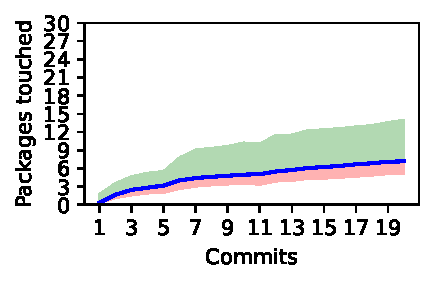
\includegraphics[width=\textwidth]{sections/results/packages/time_series_components_touched.packages.sustained.founder.commits_20.pdf}
    \caption{Sustained founder (n=34, $\mu$=9.32, median=4.0 \& std=6.14)}
    \label{figure.sections/results/packages/time_series_components_touched.packages.sustained.founder.commits_20.pdf}
  \end{subfigure}
  \begin{subfigure}[b]{0.45\textwidth}
    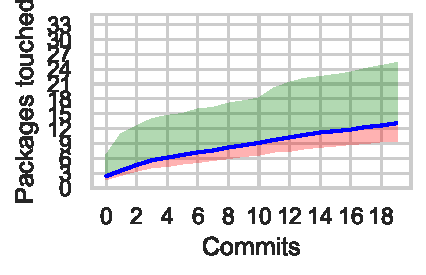
\includegraphics[width=\textwidth]{sections/results/packages/time_series_components_touched.packages.sustained.later.joiner.commits_20.pdf}
    \caption{Sustained later joiner (n=203, $\mu$=13.06, median=6.0 \& std=9.14)}
    \label{figure.sections/results/packages/time_series_components_touched.packages.sustained.later.joiner.commits_20.pdf}
  \end{subfigure}
\caption{A time series for the twenty (20) commits, sustained developers, with the average mean (blue line), packages touched (y-axis) against the number of commits (x-axis) for two (2) developer categories. Green is the standard deviation above the mean, and pink is the standard deviation below the mean.} 
\end{figure}
\clearpage 
\begin{figure}
  \centering 
  \begin{subfigure}[b]{0.45\textwidth}
    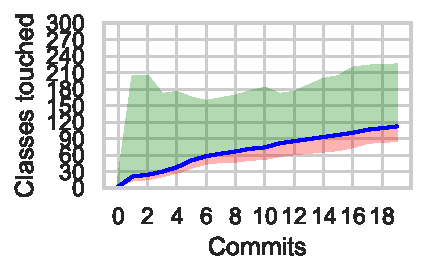
\includegraphics[width=\textwidth]{sections/results/classes/time_series_components_touched.classes.sustained.founder.commits_20.pdf}
    \caption{Sustained founder (n=34, $\mu$=107.5, median=30.0 \& std=91.26)}
    \label{figure.sections/results/classes/time_series_components_touched.classes.sustained.founder.commits_20.pdf}
  \end{subfigure}
  \begin{subfigure}[b]{0.45\textwidth}
    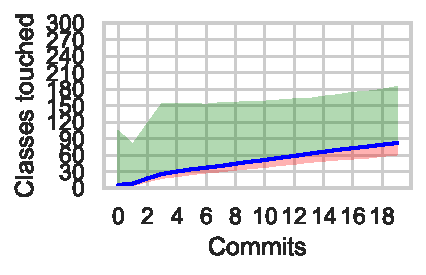
\includegraphics[width=\textwidth]{sections/results/classes/time_series_components_touched.classes.sustained.later.joiner.commits_20.pdf}
    \caption{Sustained later joiner (n=203, $\mu$=81.91, median=27.0 \& std=72.01)}
    \label{figure.sections/results/classes/time_series_components_touched.classes.sustained.later.joiner.commits_20.pdf}
  \end{subfigure}
\caption{A time series for the twenty (20) commits, sustained developers, with the average mean (blue line), classes touched (y-axis) against the number of commits (x-axis) for two (2) developer categories. Green is the standard deviation above the mean, and pink is the standard deviation below the mean.} 
\end{figure}
\clearpage 
\begin{figure}
  \centering 
  \begin{subfigure}[b]{0.45\textwidth}
    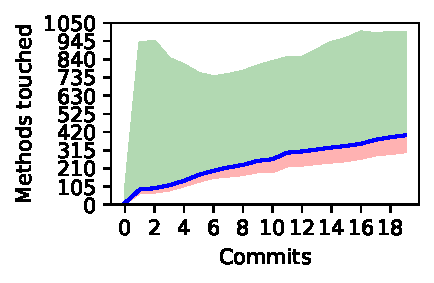
\includegraphics[width=\textwidth]{sections/results/methods/time_series_components_touched.methods.sustained.founder.commits_20.pdf}
    \caption{Sustained founder (n=34, $\mu$=401.24, median=85.5 \& std=426.09)}
    \label{figure.sections/results/methods/time_series_components_touched.methods.sustained.founder.commits_20.pdf}
  \end{subfigure}
  \begin{subfigure}[b]{0.45\textwidth}
    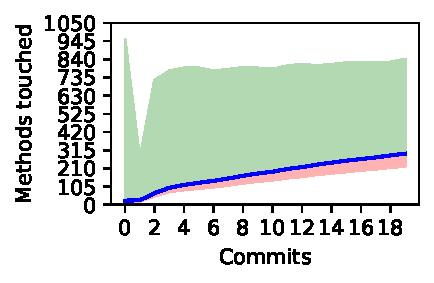
\includegraphics[width=\textwidth]{sections/results/methods/time_series_components_touched.methods.sustained.later.joiner.commits_20.pdf}
    \caption{Sustained later joiner (n=203, $\mu$=295.1, median=79.0 \& std=349.63)}
    \label{figure.sections/results/methods/time_series_components_touched.methods.sustained.later.joiner.commits_20.pdf}
  \end{subfigure}
\caption{A time series for the twenty (20) commits, sustained developers, with the average mean (blue line), methods touched (y-axis) against the number of commits (x-axis) for two (2) developer categories. Green is the standard deviation above the mean, and pink is the standard deviation below the mean.} 
\end{figure}
\clearpage 
